\documentclass[14pt,a4paper,report]{report}
\usepackage[a4paper, mag=1000, left=2.5cm, right=1cm, top=2cm, bottom=2cm, headsep=0.7cm, footskip=1cm]{geometry}
\usepackage[utf8]{inputenc}
\usepackage[english,russian]{babel}
\usepackage{indentfirst}
\usepackage[dvipsnames]{xcolor}
\usepackage[colorlinks]{hyperref}
\usepackage{listings} 
\usepackage{fancyhdr}
\usepackage{caption}
\usepackage{amsmath}
\usepackage{latexsym}
\usepackage{graphicx}
\usepackage{amsmath}
\usepackage{booktabs}
\usepackage{array}
\hypersetup{
	colorlinks = true,
	linkcolor  = black
}

\usepackage{titlesec}
\titleformat{\chapter}
{\Large\bfseries} % format
{}                % label
{0pt}             % sep
{\huge}           % before-code


\DeclareCaptionFont{white}{\color{white}} 

% Listing description
\usepackage{listings} 
\DeclareCaptionFormat{listing}{\colorbox{gray}{\parbox{\textwidth}{#1#2#3}}}
\captionsetup[lstlisting]{format=listing,labelfont=white,textfont=white}
\lstset{ 
	% Listing settings
	inputencoding = utf8,			
	extendedchars = \true, 
	keepspaces = true, 			  	 % Поддержка кириллицы и пробелов в комментариях
	language = C++,            	 	 % Язык программирования (для подсветки)
	basicstyle = \small\sffamily, 	 % Размер и начертание шрифта для подсветки кода
	numbers = left,               	 % Где поставить нумерацию строк (слева\справа)
	numberstyle = \tiny,          	 % Размер шрифта для номеров строк
	stepnumber = 1,               	 % Размер шага между двумя номерами строк
	numbersep = 5pt,              	 % Как далеко отстоят номера строк от подсвечиваемого кода
	backgroundcolor = \color{white}, % Цвет фона подсветки - используем \usepackage{color}
	showspaces = false,           	 % Показывать или нет пробелы специальными отступами
	showstringspaces = false,    	 % Показывать или нет пробелы в строках
	showtabs = false,           	 % Показывать или нет табуляцию в строках
	frame = single,              	 % Рисовать рамку вокруг кода
	tabsize = 2,                  	 % Размер табуляции по умолчанию равен 2 пробелам
	captionpos = t,             	 % Позиция заголовка вверху [t] или внизу [b] 
	breaklines = true,           	 % Автоматически переносить строки (да\нет)
	breakatwhitespace = false,   	 % Переносить строки только если есть пробел
	escapeinside = {\%*}{*)}      	 % Если нужно добавить комментарии в коде
}

\begin{document}

\def\contentsname{Содержание}

% Titlepage
\begin{titlepage}
	\begin{center}
		\textsc{Санкт-Петербургский Политехнический 
			Университет Петра Великого\\[5mm]
			Кафедра компьютерных систем и программных технологий}
		
		\vfill
		
		\textbf{Отчёт по курсовой работе\\[3mm]
			Курс: «Параллельные вычисления»\\[3mm]
			Тема: «Расчет суммы чисел для каждой вершины дерева»\\[35mm]
			}
	\end{center}
	
	\hfill
	\begin{minipage}{.5\textwidth}
		Выполнил студент:\\[2mm] 
		Бояркин Никита Сергеевич\\
		Группа: 13541/3\\[5mm]
		
		Проверил:\\[2mm] 
		Стручков Игорь Вячеславович
	\end{minipage}
	\vfill
	\begin{center}
		Санкт-Петербург\\ \the\year\ г.
	\end{center}
\end{titlepage}

% Contents
\tableofcontents
\clearpage

\chapter{Курсовая работа}

\section{Цель работы}

Целью данной работы является получение студентами навыков создания многопоточных программ с использованием интерфейсов POSIX Threads, OpenMP и MPI.

\section{Программа работы}

\begin{itemize}
	\item Для алгоритма из полученного задания написать последовательную программу на языке C или С++, реализующую этот алгоритм.
	\item Для созданной последовательной программы необходимо написать 3-5 тестов, которые покрывают основные варианты функционирования программы. Для создания тестов можно воспользоваться механизмом Unit-тестов среды NetBeans, или описать входные тестовые данные в файлах. При использовании NetBeans необходимо в свойствах проекта установить ключ компилятора -pthread.
	\item Проанализировать полученный алгоритм, выделить части, которые могут быть распараллелены, разработать структуру параллельной программы. Определить количество используемых потоков, а также правила и используемые объекты синхронизации.
	\item Согласовать разработанную структуру и детали реализации параллельной программы с преподавателем.
	\item Написать код параллельной программы и проверить ее корректность на созданном ранее наборе тестов. При необходимости найти и исправить ошибки.
	\item Провести эксперименты для оценки времени выполнения последовательной и параллельной программ. Проанализировать полученные результаты.
	\item Сделать общие выводы по результатам проделанной работы: Различия между способами проектирования последовательной и параллельной реализаций алгоритма, Возможные способы выделения параллельно выполняющихся частей, Возможные правила синхронизации потоков, Сравнение времени выполнения последовательной и параллельной программ, Принципиальные ограничения повышения эффективности параллельной реализации по сравнению с последовательной.
\end{itemize}

\section{Индивидуальное задание}

\textbf{Вариант №6}

Вершины дерева размечены числовыми значениями. Для каждой вершины рассчитать сумму чисел всех вершин, для которых данная вершина является корнем.

Средство распараллеливания -- \textbf{MPI}.

\section{Компиляция и компоновка проекта}

В качестве среды разработки используется IDE Netbeans, в качестве компилятора и компоновщика используется специальная обертка над компилятором g++ и компоновщиком ld, которая запускает их с определенными флагами командной строки для осуществления распараллеливания MPI:

\lstinputlisting{listings/0k.log}

Дополнительные флаги, необходимые для компиляции проекта:

\lstinputlisting{listings/0f.log}

Для запуска многопроцессного приложения MPI используется специальная команда, если ее не использовать, приложение запустится на одном процессе:

\lstinputlisting{listings/0m.log}

\section{Ход работы}

\subsection{Формализация задачи и детали реализации}

\begin{itemize}
	\item Дерево не бинарное, так как это явно не указывается в формулировке задания.
	\item Реализация дерева -- собственный класс на языке C++.
	\item Расчет суммы чисел всех вершин, для которых данная вершина является корнем, является задачей нахождения нового дерева с вершинами равными этим суммам, пример представлен на рис. \ref{image:1}.
	\item Различные алгоритмы реализации расчета дерева сумм (рекурсивная, последовательная, многопоточная pthread, многопроцессная MPI) являются функциями, вызываемыми на объекте дерева.
	\item Численные значения вершин дерева -- числа с плавающей точкой, могут быть отрицательными.
	\item Точность значений с плавающей точкой при получении дерева сумм может теряться для упрощения задачи.
	\item Объект дерева задается из символьной строки и может быть конвертирован в символьную строку через функции, вызываемые непосредственно на объекте дерева или статически на классе.
\end{itemize}

\begin{figure}[h!]
	\centering
	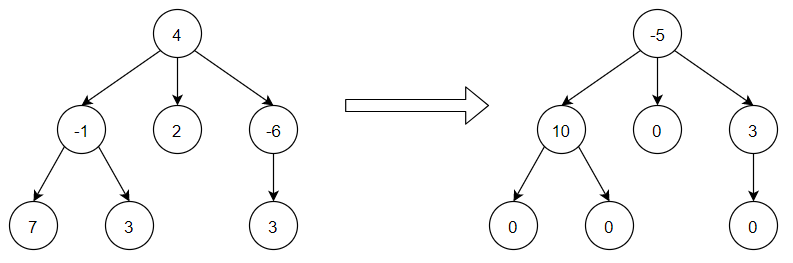
\includegraphics[scale = 0.7]{images/1.png}
	\caption{Нахождение нового дерева с суммами вершин}
	\label{image:1}
\end{figure}

\subsection{Разработка структуры данных и общих функций}

Класс дерева tree имеет достаточно несложную реализацию:

\lstinputlisting{listings/1.cpp}

На классе дерева есть подкласс вершины node. Каждая вершина содержит собственное численное значение и набор вершин для которых данная вершина является корнем.

Само дерево содержит только корневую вершину.

Задать дерево можно из символьной строки в определенном формате:

\begin{verbatim}
4(-1(7(),3()),2(),-6(3()))
\end{verbatim}

Данная строка соответствует следующему дереву:

\begin{figure}[h!]
	\centering
	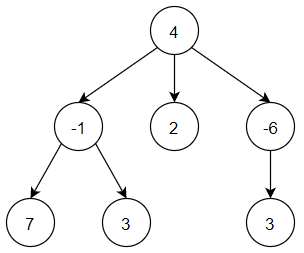
\includegraphics[scale = 0.7]{images/2.png}
	\caption{Пример дерева из символьной строки}
	\label{image:2}
\end{figure}

Реализация функции перевода строки в дерево:

\lstinputlisting{listings/1fs.cpp}

Функция целенаправленно была реализована без использования рекурсии, для того, чтобы можно было быстро парсить большие деревья.

\subsection{Разработка последовательной реализации}

Самой простой реализацией является рекурсивная:

\lstinputlisting{listings/2r.cpp}

Проблемой рекурсии в C++ является то, что стек быстро заканчивается, а компилятор не всегда распознает рекурсию и не разворачивает ее в цикл.

Таким образом для больших деревьев намного лучше подходит реализация при помощи цикла:

\lstinputlisting{listings/2c.cpp}

Для разворачивания рекурсии в цикл был добавлен собственный стек, который хранит указатели на вершину и ее корень, для последующего суммирования.

\subsection{Разработка многопоточной реализации при помощи pthread}

Распараллеливание подобного алгоритма подразумевает создание нового потока для каждой вершины дерева. Однако, такая реализация абсолютно неэффективна, намного быстрее и эффективнее по памяти будет реализация с ограничением количества работающих потоков до определенного значения. Кроме того, каждый поток, отрабатывая собственную вершину не должен ожидать другие, а должен переходить к следующей необработанной вершине.

Распараллеленный алгоритм будет строиться на основе реализации при помощи цикла из предыдущего пункта. Таким образом должны быть синхронизированы следующие операции, связанные с общими данными:

\begin{itemize}
	\item Добавление и считывание данных из стека вершин.
	\item Обнуление значения вершины, запись суммы в значение вершины.
	\item Инкрементация и декрементация количества работающих потоков, проверка на количество работающих потоков.
\end{itemize}

Данные операции могут быть синхронизированы при помощи трех мьютексов.

В связи с особенностью библиотеки pthread необходимо разработать структуру, содержащую указатели на все необходимые общие данные. Эта структура передается как единственный аргумент каждому из потоков. Кроме того необходимо создать статическую функцию, которая будет вызываться в потоках:

\lstinputlisting{listings/3s.cpp}

Максимальное количество потоков выбивается равным количеству доступных CPU при помощи функции std::thread::hardware\_concurrency() для  обеспечения наилучшей производительности \cite{cite-best-thread-count} Многопоточная реализация алгоритма:

\lstinputlisting{listings/3r.cpp}

\subsection{Разработка многопроцессной реализации при помощи MPI}

Message Passing Interface (MPI) -- программный интерфейс для передачи информации, который позволяет обмениваться сообщениями между процессами, выполняющими одну задачу \cite{cite-mpi} Основным средством коммуникации между процессами в MPI является передача сообщений друг другу.

В первую очередь MPI ориентирован на системы с распределенной памятью, то есть когда затраты на передачу данных велики, в то время как OpenMP ориентирован на системы с общей памятью (многоядерные с общим кешем). Обе технологии могут использоваться совместно, чтобы оптимально использовать в кластере многоядерные системы.

К сожалению, данная задача совсем не подходит для распараллеливания при помощи MPI \cite{cite-tree-traversal-mpi}. Адресные пространства каждого из процессов MPI разделены, поэтому не получится обходить дерево подобным образом. MPI хорошо подходит для размещения или обмена простыми общими данными: целыми числами, числами с плавающей точкой, массивами чисел и др. Однако, поместить в разделяемую память подобный объект дерева не получится, поэтому распараллелить такой алгоритм черезвычайно сложно и скорее всего полученная реализация будет намного медленнее реализаций, описанных до этого. Для задач, задействующих большие объемы неструктурированной общей памяти, лучше подходит OpenMP.

В связи с этим, было принято решение распараллелить алгоритм расчета экспоненты для демонстрации особенностей работы с MPI:

\lstinputlisting{listings/4r.cpp}

Заметим, что в реализацим подсчета экспоненты при помощи MPI на каждый процесс приходится в N раз меньше итераций цикла, где N это количество процессов.

Функции не задействующие MPI должны вызываться только на нулевом ранге (обеспечение единственности процесса), а задействующие должны вызываться для всех процессов:

\lstinputlisting{listings/4m.cpp}

В результате работы было выведено:

\lstinputlisting{listings/4m.log}

Таким образом, задача была распараллелена на шесть процессов, в результате чего был получен правильный результат вычисления экспоненты.

\subsection{Тестирование}

\subsubsection{Тестирование производительности MPI}

Для тестирования производительности MPI на примере функции вычисления экспоненты разработаем тест, который замеряет время выполнения с высокой точностью через функции класса std::chrono::high\_resolution\_clock.

\lstinputlisting{listings/5.1.cpp}

\clearpage

Результаты тестирования производительности вычисления экспоненты:

\begin{table}[h!]
	\centering
	\bgroup
	\def\arraystretch{1}
	\begin{tabular}{ | m{0.8cm} | m{2.0cm} | m{1.8cm} | m{2.6cm} | m{2.6cm} | }
		\hline
		№ & precision & iterations & Simple, ms & MPI, ms \\ \hline
		1 & 10 & 200 & 0.042692 & 152.628 \\ \hline
		2 & 100 & 20 & 1.21271 & 8.19007 \\ \hline
		3 & 5000 & 10 & 7790.65 & 1656.67 \\ \hline
		4 & 10000 & 2 & 10197.7 & 1923.33 \\
		\hline
	\end{tabular}
	\egroup
\end{table}

Как и ожидалось, с увеличением сложности вычисления экспоненты (увеличением точности) распараллеливание MPI дает все большее преимущество по сравнению с простым алгоритмом.

Для подсчета статистики разработаем скрипт на языке python, который принимает путь к файлу с выборкой как аргумент командной строки и выводит статистические данные, такие как мат ожидание, дисперсия, радиус и интервал:

\lstinputlisting{listings/5s.py}

Вычислим статистические данные на наборе значений:

\begin{table}[h!]
	\centering
	\bgroup
	\def\arraystretch{1}
	\begin{tabular}{ | m{0.95cm} | m{1.5cm} | m{1.5cm} | m{2.2cm} | m{2.2cm} | m{2.2cm} | m{4.1cm} | }
		\hline
		 & precision & iterations & mean, ms & dispersion & radius, ms & interval, ms \\ \hline
		Simple & 10 & 200 & 0.000255 & 0.000000 & 0.000000 & [0.000255, 0.000255] \\ \hline
		MPI & 10 & 200 & 0.113854 & 0.477850 & 0.005712 & [0.108142, 0.119566] \\ \hline \hline
		Simple & 100 & 20 & 0.019282 & 0.000000 & 0.000011 & [0.019272, 0.019293] \\ \hline
		MPI & 100 & 20 & 0.567151 & 5.676893 & 0.205994 & [0.361158, 0.773145] \\ \hline \hline
		Simple & 5000 & 10 & 699.0373 & 3307.407968 & 10.542245 & [688.495055, 709.579545] \\ \hline
		MPI & 5000 & 10 & 156.2293 & 1221.598 & 6.40698 & [149.822320, 162.636280] \\ \hline \hline
		Simple & 10000 & 2 & 4075.785000 & 4458.512450 & 210.791203 & [3864.993797, 4286.576203] \\ \hline
		MPI & 10000 & 2 & 886.405500 & 10.511112 & 10.234858 & [876.170642, 896.640358] \\
		\hline
	\end{tabular}
	\egroup
\end{table}

\clearpage

Вычислим зависимость от количества процессов MPI для точности 4000 и числа измерений 100 (вычисление производится на процессоре с 6 ядрами):

\begin{table}[h!]
	\centering
	\bgroup
	\def\arraystretch{1}
	\begin{tabular}{ | m{2.1cm} | m{1.8cm} | m{1.8cm} | m{2.1cm} | m{2.1cm} | m{4.1cm} | }
		\hline
		process count & total, ms & mean, ms & dispersion & radius, ms & interval, ms \\ \hline
		1 			  & 29908.916 & 299.08916 & 41.855861 & 0.107421 & [298.981739, 299.196581] \\ \hline
		2 			  & 15151.683 & 151.51683 & 37.224975 & 0.101304 & [151.415526, 151.618134] \\ \hline
		4 			  & 8441.8148 & 84.418148 & 86.420509 & 0.154354 & [84.263794, 84.572502] \\ \hline
		6 			  & 7938.9617 & 79.38961 & 330.026356 & 0.301637 & [79.087980, 79.691254] \\ \hline
		8 			  & 8681.0363 & 86.810363 & 152.559181 & 0.205083 & [86.605280, 87.015446] \\ \hline
		10 			  & 7435.9975 & 74.359975 & 103.587356 & 0.168991 & [74.190984, 74.528966] \\ \hline
		12 			  & 7653.9843 & 76.539843 & 184.187987 & 0.225341 & [76.314502, 76.765184] \\
		\hline
	\end{tabular}
	\egroup
\end{table}

Построим график зависимости времени выполнения (вертикальная ось в секундах) от количества процессов(горизонтальная ось):

\begin{figure}[h!]
	\centering
	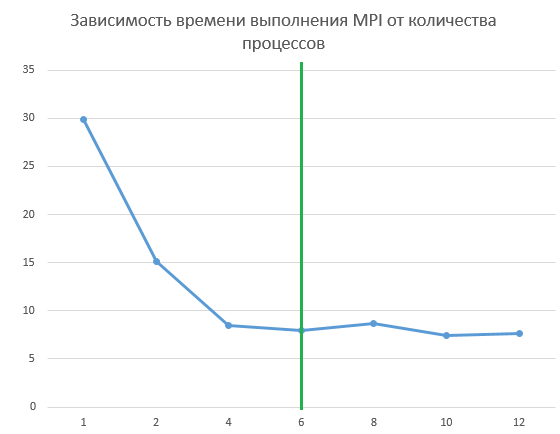
\includegraphics[scale = 0.7]{images/3.png}
	\caption{Зависимость времени выполнения MPI от количества процессов}
	\label{image:3}
\end{figure}

Зеленым отмечено количество ядер в текущем процессоре. Можно заметить, что наиболее значимый выигрыш в производительности наблюдается при переходе от одного процесса к двум (практически в два раза). Также неплохой выигрыш наблюдается при переходе от двух процессов к четырем. Последующее наращивание количества процессов не сильно улучшает производительность.

\subsubsection{Тестирование алгоритмов на дереве}

Тестирование алгоритмов на дереве (рекурсивного, последовательного и многопоточного) производится на трех деревьях с различным числом вершин:

\begin{itemize}
	\item Маленькое дерево -- 36 вершин.
	\item Среднее дерево -- 7014 вершин.
	\item Большое дерево -- 598528 вершин.
\end{itemize}

Первый тест основывается на тезисе, что результат всех трех алгоритмов на одном и том же дереве должен быть одинаковым:

\lstinputlisting{listings/5.2.cpp}

Подобный тест повторяется для всех трех тестовых деревьев.

Второй тест основывается на тезисе, что если все три алгоритма повторить дважды (или N раз) на одном и том же дереве, то должен получиться одинаковый результат:

\lstinputlisting{listings/5.3.cpp}

Подобный тест также повторяется для всех трех тестовых деревьев.

Тестирование производительности также производится замерами времени выполнения при нескольких итерациях:

\lstinputlisting{listings/5.4.cpp}

Результаты тестирования производительности:

\begin{table}[h!]
	\centering
	\bgroup
	\def\arraystretch{1}
	\begin{tabular}{ | m{0.8cm} | m{2.0cm} | m{1.8cm} | m{2.8cm} | m{2.6cm} | m{2.6cm} | }
		\hline
		№ & nodes & iterations & Recursive, ms & Cyclic, ms & Pthread, ms \\ \hline
		1 & 36 & 20000 & 720.38 & 454.585 & 13467.2 \\ \hline
		2 & 7014 & 200 & 2914.3 & 957.112 & 1742.87 \\ \hline
		3 & 598528 & 2 & 9870.23 & 809.911 & 1182.03 \\
		\hline
	\end{tabular}
	\egroup
\end{table}

Таким образом, рекурсивная реализация ожидаемо является самой медленной из трех.

Распараллеленная реализация оказалась медленней реализации через цикл. Это объясняется тем, что задача выполняемая на каждой вершине слишком простая (сумма двух чисел), а на контекстные переключения уходит больше времени, чем выигрывается.

Вычислим статистические данные на наборе значений:

\begin{table}[h!]
	\centering
	\bgroup
	\def\arraystretch{1}
	\begin{tabular}{ | m{1.5cm} | m{1.5cm} | m{1.5cm} | m{2.0cm} | m{2.0cm} | m{2.0cm} | m{4.1cm} | }
		\hline
		& nodes & iterations & mean, ms & dispersion & radius, ms & interval, ms \\ \hline
		Recursive & 36 & 20000 & 0.035285 & 0.002819 & 0.000004 & [0.035281, 0.035290] \\ \hline
		Cyclic & 36 & 20000 & 0.024768 & 0.005636 & 0.000006 & [0.024761, 0.024774] \\ \hline
		Pthread & 36 & 20000 & 0.618434 & 0.798031 & 0.000073 & [0.618360, 0.618507] \\ \hline \hline
		Recursive & 7014 & 200 & 13.127591 & 1.725761 & 0.010855 & [13.116737, 13.138446] \\ \hline
		Cyclic & 7014 & 200 & 4.104959 & 0.004363 & 0.000546 & [4.104413, 4.105505] \\ \hline
		Pthread & 7014 & 200 & 8.087841 & 6.705221 & 0.021396 & [8.066445, 8.109236] \\ \hline \hline
		Recursive & 598528 & 2 & 4794.750000 & 9253.440800 & 303.675053 & [4491.074947, 5098.425053] \\ \hline
		Cyclic & 598528 & 2 & 399.068000 & 536.543282 & 73.123988 & [325.944012, 472.191988] \\ \hline
		Pthread & 598528 & 2 & 585.838500 & 4573.791724 & 213.498920 & [372.339580, 799.337420] \\
		\hline
	\end{tabular}
	\egroup
\end{table}

Высчитывать зависимость от количества потоков бессмысленно, так как количество потоков с такой простой задачей никак не повлияет на результат.

Усложним задачу для каждой вершины добавив задержку во все реализации алгоритма:

\lstinputlisting{listings/5.5.cpp}

Для многопоточной реализации важно добавить задержку в область, не синхронизируемую мьютексами, так как выигрыш от многопоточной реализации достигается только вычислениями, которые можно выполнять параллельно без ущерба для целостности.

Результаты тестирования производительности с добавлением искусственной задержки:

\begin{table}[h!]
	\centering
	\bgroup
	\def\arraystretch{1}
	\begin{tabular}{ | m{0.8cm} | m{2.0cm} | m{1.8cm} | m{2.8cm} | m{2.6cm} | m{2.6cm} | }
		\hline
		№ & nodes & iterations & Recursive, ms & Cyclic, ms & Pthread, ms \\ \hline
		1 & 36 & 20000 & 3745.25 & 3501.24 & 14416.3 \\ \hline
		2 & 7014 & 200 & 8955.39 & 7005.93 & 2999.5 \\ \hline
		3 & 598528 & 2 & 15390.8 & 6068.39 & 2551.58 \\
		\hline
	\end{tabular}
	\egroup
\end{table}

Рекурсивная реализация все еще наиболее медленная, зато многопоточная стала намного быстрее относительно других. Для каждого потока появилась реальная задача, которую можно выполнять параллельно, поэтому контекстные переключения уже не так значительно влияют на общую производительность.

Вычислим статистические данные на наборе значений:

\begin{table}[h!]
	\centering
	\bgroup
	\def\arraystretch{1}
	\begin{tabular}{ | m{1.5cm} | m{1.5cm} | m{1.5cm} | m{2.0cm} | m{2.0cm} | m{2.0cm} | m{4.1cm} | }
		\hline
		& nodes & iterations & mean, ms & dispersion & radius, ms & interval, ms \\ \hline
		Recursive & 36 & 20000 & 0.187652 & 0.004227 & 0.000005 & [0.187647, 0.187658] \\ \hline
		Cyclic & 36 & 20000 & 0.174525 & 0.000037 & 0.000001 & [0.174524, 0.174525] \\ \hline
		Pthread & 36 & 20000 & 0.527426 & 0.380192 & 0.000051 & [0.527375, 0.527477] \\ \hline \hline
		Recursive & 7014 & 200 & 44.077959 & 4.952748 & 0.018389 & [44.059570, 44.096347] \\ \hline
		Cyclic & 7014 & 200 & 34.709729 & 0.062914 & 0.002073 & [34.707656, 34.711801] \\ \hline
		Pthread & 7014 & 200 & 12.814718 & 8.034588 & 0.023421 & [12.791297, 12.838139] \\ \hline \hline
		Recursive & 598528 & 2 & 7347.590 & 9549.620 & 308.496709 & [7039.093291, 7656.086709] \\ \hline
		Cyclic & 598528 & 2 & 2988.885 & 456.926450 & 67.480865 & [2921.404135, 3056.365865] \\ \hline
		Pthread & 598528 & 2 & 1053.120000 & 2000.913800 & 141.212025 & [911.907975, 1194.332025] \\
		\hline
	\end{tabular}
	\egroup
\end{table}

Можно заметить, что у многопоточного алгоритма дисперсия существенно выше чем у других алгоритмов, даже при том, что среднее значение наименьшее.

\clearpage

Вычислим зависимость от количества потоков Ptherad алгоритма для дерева с количеством вершин 598528 и числа измерений 30 (вычисление производится на процессоре с 6 ядрами):

\begin{table}[h!]
	\centering
	\bgroup
	\def\arraystretch{1}
	\begin{tabular}{ | m{2.1cm} | m{1.8cm} | m{1.8cm} | m{2.1cm} | m{2.1cm} | m{4.1cm} | }
		\hline
		threads count & total, ms & mean, ms & dispersion & radius, ms & interval, ms \\ \hline
		1 			  & 92572.1 & 3085.736667 & 669.155106 & 1.465102 & [3084.271564, 3087.201769] \\ \hline
		2 			  & 32923.23 & 1097.441 & 18467.619761 & 7.696797 & [1089.744203, 1105.137797] \\ \hline
		4 			  & 31187.036 & 1039.567867 & 2430.774867 & 2.792396 & [1036.775471, 1042.360262] \\ \hline
		6 			  & 32249.43 & 1074.981 & 730.856823 & 1.531161 & [1073.449839, 1076.512161] \\ \hline
		8 			  & 35215.12 & 1173.837333 & 4114.585951 & 3.633019 & [1170.204314, 1177.470352] \\ \hline
		10 			  & 34528.08 & 1150.936 & 2198.330673 & 2.655529 & [1148.280471, 1153.591529] \\ \hline
		12 			  & 33508.83 & 1116.961 & 801.721989 & 1.603675 & [1115.357325, 1118.564675] \\
		\hline
	\end{tabular}
	\egroup
\end{table}

Построим график зависимости времени выполнения (вертикальная ось в секундах) от количества потоков (горизонтальная ось):

\begin{figure}[h!]
	\centering
	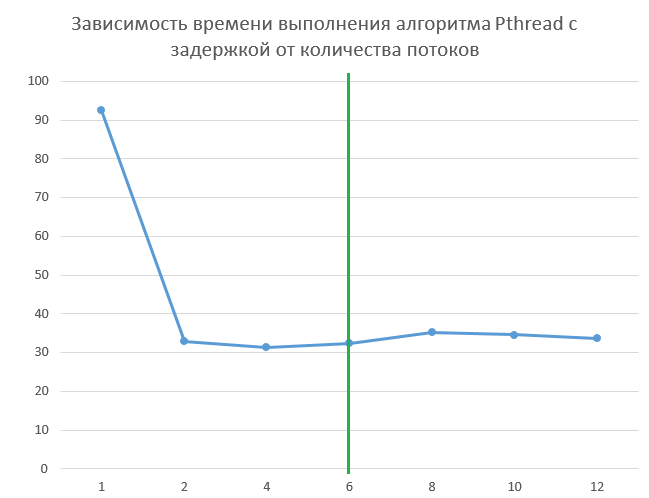
\includegraphics[scale = 0.55]{images/4.png}
	\caption{Зависимость времени выполнения алгоритма Pthread от количества потоков}
	\label{image:4}
\end{figure}

Уже при двух потоках время выполнения практически оптимальное, однако дисперсия на двух потоках очень большая и постепенно уменьшается с наращиванием количества потоков до шести, что хорошо иллюстрируется следующим графиком:

\begin{figure}[h!]
	\centering
	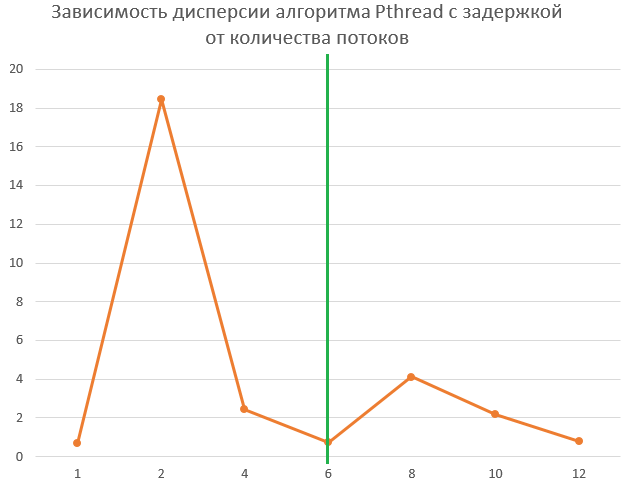
\includegraphics[scale = 0.55]{images/5.png}
	\caption{Зависимость дисперсии алгоритма Pthread от количества потоков}
	\label{image:5}
\end{figure}

\section{Вывод}

В ходе работы было разработано несколько алгоритмов для нахождения дерева сумм: рекурсивный, циклический и многопоточный (с ограничением количества потоков и без). Многопоточный алгоритм без ограничения количества потоков не рассматривался в работе ввиду общей неэффективности и непрохождении тестов на больших деревьях. Кроме того, был разработан демонстрационный MPI проект по поиску экспоненты с заданной точностью и его последующем тестировании.

Рекурсивная реализация алгоритмов плоха не только тем, что стек может переполниться, но и показывает в целом меньшую производительность, чем такой же алгоритм, реализованный через цикл.

Многопоточная реализация не является общим решением: приходится жертвовать производительностью на небольших данных, кроме того потоки занимают большое количество памяти. Многопоточную реализацию имеет смысл применять, когда для каждого потока есть трудоемкая подзадача, которую можно выполнять параллельно, чтобы контекстные переключения не так значительно влияли на общую производительность. Кроме того, имеет смысл ограничить количество потоков равным количеству доступных CPU для наилучшей производительности.

Для задач с необходимостью доступа к сложноструктурированной общей памяти MPI не очень подходит. Это объясняется тем, что деревья, графы и подобные структуры в C++ весьма тяжело положить в разделяемую память, поэтому придется придумывать сложные неэффективные способы распараллеливания с передачей стандартных сообщений MPI. Однако, MPI отлично подходит для распараллеливания математических алгоритмов по типу вычисления экспоненты или числа пи, кроме того, MPI широко используется для распараллеливания программ для кластеров и суперкомпьютеров.

Наиболее значимый выигрыш в производительности вычисления экспоненты MPI наблюдается при переходе от одного процесса к двум (практически в два раза). Также неплохой выигрыш наблюдается при переходе от двух процессов к четырем. Последующее наращивание количества процессов не сильно улучшает производительность.

\bibliography{thesis}
\bibliographystyle{ugost2008}

\end{document}